\documentclass[11pt,a4paper,oneside]{book}

% -----------------------------------------------------------------------------
% Packages
% -----------------------------------------------------------------------------
\usepackage[utf8]{inputenc}
\usepackage[T1]{fontenc}
\usepackage{lmodern}
\usepackage{microtype}
\usepackage[margin=1in,headheight=24pt]{geometry}
\usepackage{graphicx}
\usepackage{xcolor}
\usepackage{listings}
\usepackage{tcolorbox}
\tcbuselibrary{skins,breakable}
\usepackage{titlesec}
\usepackage{fancyhdr}
\usepackage{booktabs}
\usepackage{tabularx}
\usepackage{hyperref}
\usepackage{bookmark}

% -----------------------------------------------------------------------------
% Color Palette
% -----------------------------------------------------------------------------
\definecolor{brandblue}{RGB}{26, 115, 232}     % Google Blue
\definecolor{darkslate}{RGB}{30, 41, 59}       % Deep Slate
\definecolor{accentpurple}{RGB}{124, 58, 237}  % Vibrant Violet
\definecolor{tealglow}{RGB}{13, 148, 136}      % Cyan Teal
\definecolor{warningamber}{RGB}{217, 119, 6}   % Amber
\definecolor{crimsonred}{RGB}{225, 29, 72}     % Crimson
\definecolor{codebg}{RGB}{245, 247, 250}       % Light Gray/Blue
\definecolor{codeborder}{RGB}{203, 213, 225}   % Slate Border

% -----------------------------------------------------------------------------
% Hyperref Settings
% -----------------------------------------------------------------------------
\hypersetup{
    colorlinks=true,
    linkcolor=brandblue,
    citecolor=accentpurple,
    urlcolor=tealglow,
    pdftitle={Mastering Antigravity: The Definitive Guide to AI-First Software Engineering},
    pdfauthor={Sudheer K. Mohammed},
    pdfsubject={Software Engineering, Autonomous AI Agents, Google Antigravity, Prompt Engineering, Goal Architecture},
    pdfkeywords={Antigravity, AI Agents, LLM, Gemini, Software Engineering, DevTools, CLI, SDK, IDE, Prompts, Goals}
}

% -----------------------------------------------------------------------------
% Header & Footer Styling
% -----------------------------------------------------------------------------
\pagestyle{fancy}
\fancyhf{}
\fancyhead[L]{\small\color{darkslate}\textbf{\leftmark}}
\fancyhead[R]{\small\color{brandblue}\textbf{Mastering Antigravity}}
\fancyfoot[C]{\small\thepage}
\renewcommand{\headrulewidth}{0.4pt}
\renewcommand{\footrulewidth}{0pt}

% -----------------------------------------------------------------------------
% Chapter & Section Styling
% -----------------------------------------------------------------------------
\titleformat{\chapter}[display]
  {\normalfont\bfseries\color{darkslate}}
  {\filleft\Huge\color{brandblue}Chapter \thechapter}
  {1ex}
  {\titlerule[2pt]\vspace{2ex}\huge\color{darkslate}}
  [\vspace{1ex}\titlerule]

\titleformat{\section}
  {\normalfont\Large\bfseries\color{brandblue}}
  {\thesection}{1em}{}

\titleformat{\subsection}
  {\normalfont\large\bfseries\color{accentpurple}}
  {\thesubsection}{1em}{}

% -----------------------------------------------------------------------------
% Custom Callout Boxes (tcolorbox)
% -----------------------------------------------------------------------------
\newtcolorbox{probox}[1][]{
    enhanced,
    breakable,
    colback=codebg,
    colframe=brandblue,
    coltitle=white,
    title=\textbf{Pro Tip: #1},
    arc=4pt,
    boxrule=1.2pt,
    fonttitle=\bfseries\sffamily,
    left=10pt, right=10pt, top=8pt, bottom=8pt,
    before skip=12pt, after skip=12pt
}

\newtcolorbox{warstory}[1][]{
    enhanced,
    breakable,
    colback=codebg,
    colframe=accentpurple,
    coltitle=white,
    title=\textbf{War Story from the Trenches: #1},
    arc=4pt,
    boxrule=1.2pt,
    fonttitle=\bfseries\sffamily,
    left=10pt, right=10pt, top=8pt, bottom=8pt,
    before skip=12pt, after skip=12pt
}

\newtcolorbox{cautionbox}[1][]{
    enhanced,
    breakable,
    colback=codebg,
    colframe=crimsonred,
    coltitle=white,
    title=\textbf{Caution \& Security Warning: #1},
    arc=4pt,
    boxrule=1.2pt,
    fonttitle=\bfseries\sffamily,
    left=10pt, right=10pt, top=8pt, bottom=8pt,
    before skip=12pt, after skip=12pt
}

\newtcolorbox{conceptbox}[1][]{
    enhanced,
    breakable,
    colback=codebg,
    colframe=tealglow,
    coltitle=white,
    title=\textbf{Core Architecture Concept: #1},
    arc=4pt,
    boxrule=1.2pt,
    fonttitle=\bfseries\sffamily,
    left=10pt, right=10pt, top=8pt, bottom=8pt,
    before skip=12pt, after skip=12pt
}

\newtcolorbox{labbox}[1][]{
    enhanced,
    breakable,
    colback=codebg,
    colframe=darkslate,
    coltitle=white,
    title=\textbf{Engineering Lab Project: #1},
    arc=4pt,
    boxrule=1.2pt,
    fonttitle=\bfseries\sffamily,
    left=10pt, right=10pt, top=8pt, bottom=8pt,
    before skip=12pt, after skip=12pt
}

\newtcolorbox{promptbox}[1][]{
    enhanced,
    breakable,
    colback=codebg,
    colframe=brandblue!85!black,
    coltitle=white,
    title=\textbf{Production Prompt Template: #1},
    arc=4pt,
    boxrule=1.2pt,
    fonttitle=\bfseries\sffamily,
    left=10pt, right=10pt, top=8pt, bottom=8pt,
    before skip=12pt, after skip=12pt
}

% -----------------------------------------------------------------------------
% Listings (Code Block Styling)
% -----------------------------------------------------------------------------
\lstset{
    backgroundcolor=\color{codebg},
    basicstyle=\small\ttfamily\color{darkslate},
    keywordstyle=\bfseries\color{brandblue},
    commentstyle=\itshape\color{gray},
    stringstyle=\color{accentpurple},
    numbers=left,
    numberstyle=\tiny\color{gray},
    stepnumber=1,
    numbersep=8pt,
    frame=single,
    rulecolor=\color{codeborder},
    breaklines=true,
    breakatwhitespace=true,
    tabsize=2,
    showstringspaces=false,
    captionpos=b,
    xleftmargin=15pt,
    framexleftmargin=15pt,
    mathescape=false
}

% -----------------------------------------------------------------------------
% Document Start
% -----------------------------------------------------------------------------
\begin{document}

% -----------------------------------------------------------------------------
% Cover Page
% -----------------------------------------------------------------------------
\begin{titlepage}
    \centering
    \vspace*{0.5cm}
    
    {\Huge\textbf{\color{brandblue}MASTERING ANTIGRAVITY}}\\[0.4cm]
    {\Large\textbf{\color{darkslate}The Definitive Guide to AI-First Software Engineering}}\\[0.2cm]
    {\large\color{gray}Expanded Edition: Prompts, Goal Architecture \& The Modern AI Developer Toolkit}
    
    \vspace{1.2cm}
    
    \begin{center}
        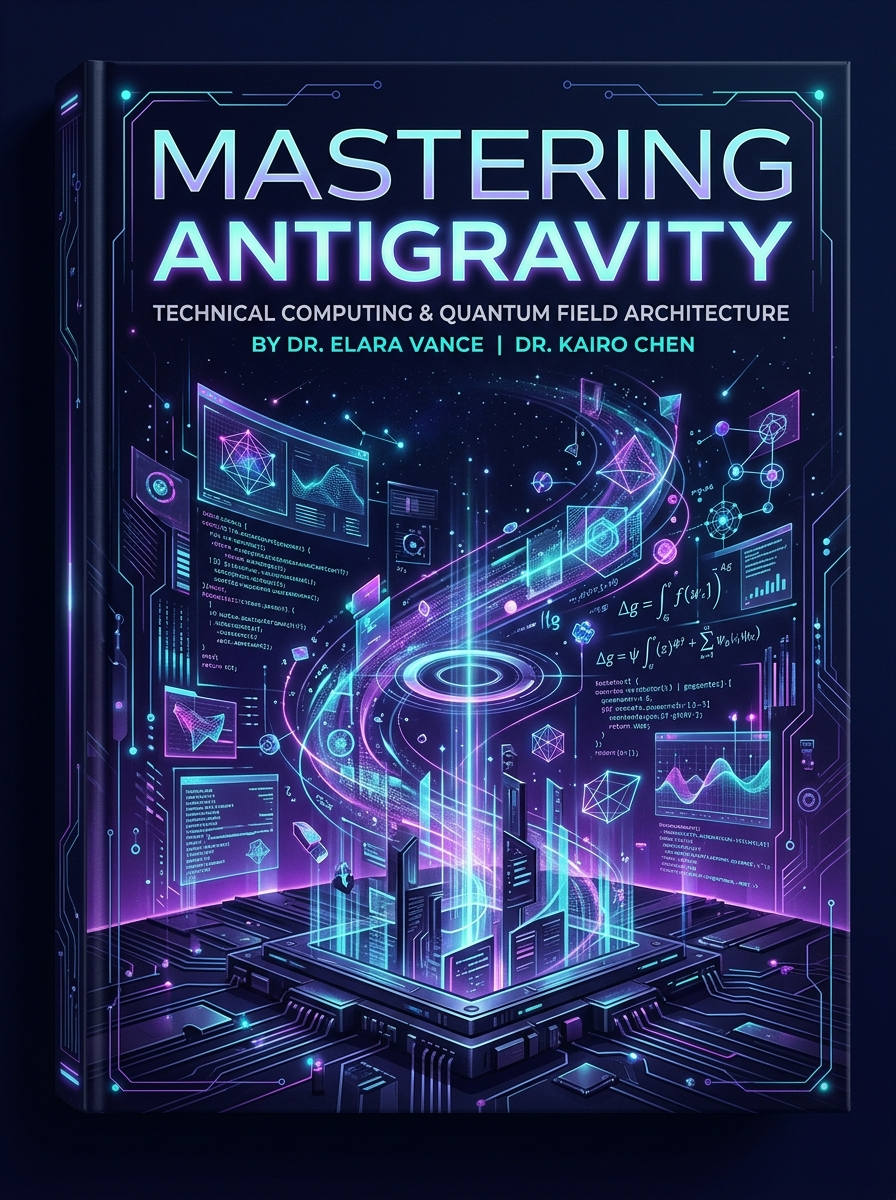
\includegraphics[width=0.65\textwidth]{images/cover.jpg}
    \end{center}
    
    \vspace{1.2cm}
    
    {\large\textbf{\color{darkslate}Sudheer K. Mohammed}}\\[0.2cm]
    {\normalsize\color{gray}Comprehensive Reference Edition $\bullet$ 2026}
    
    \vfill
\end{titlepage}

\frontmatter

% -----------------------------------------------------------------------------
% Dedication / Preface
% -----------------------------------------------------------------------------
\chapter*{Foreword: Escaping the Gravity Well}
\addcontentsline{toc}{chapter}{Foreword: Escaping the Gravity Well}

For over seven decades, software development has been bound by an inescapable law of cognitive gravity. Every line of code written demanded an equal measure of mental overhead: keeping track of transitive dependency conflicts, syntax quirks, mutating framework lifecycles, and arcane compiler flags. As codebases ballooned from tens of thousands of lines into multimillion-line monorepos, developer productivity became chained to the floor.

When LLMs emerged, early attempts simply dropped autocomplete boxes into old text editors. They were pleasant novelties, but they did not solve the fundamental crisis: software engineering is not typing; it is \textbf{reasoning, planning, executing, and verifying}.

\textbf{Google Antigravity (AGY)} represents the escape velocity. Antigravity treats artificial intelligence not as an assistant that guesses your next twenty characters, but as a \textbf{peer engineer} equipped with a sandboxed terminal, code navigation ASTs, headless browser automation, and strict safety governance.

This expanded edition is designed as the ultimate engineering manual. It does not simply explain theories: it breaks down the exact architectural differences between the **CLI**, the **IDE**, the **2.0 Desktop Canvas**, and the **Python SDK**, presents battle-tested prompt blueprints, establishes the formal mathematics of goal definition, and charts the essential skill stack required for software engineers to thrive in the agentic era.

\tableofcontents

\mainmatter

% =============================================================================
% PART I: THE GROUND FLOOR (BEGINNER)
% =============================================================================
\part{The Ground Floor (Beginner)}

\chapter{The AI-First Awakening}

\section{Beyond the Digital Typewriter}
To understand Antigravity, one must first unlearn the last twenty years of editor philosophy. The classical IDE—born of Smalltalk, refined by Eclipse, and popularized by Visual Studio Code—is built on a singular premise: \textit{a human sits at a keyboard, manually edits buffer strings, and occasionally asks external programs (compilers, linters) to evaluate those strings}.

When AI was first introduced to this paradigm, it was relegated to the status of an advanced spellchecker. Copilot-style tools operated under strict token-completion constraints: given the cursor location $L$ in document $D$, predict tokens $t_{1}, t_{2}, \dots, t_{n}$. 

This passive modality suffers from three fatal flaws:
\begin{enumerate}
    \item \textbf{Zero Architectural Intention}: The autocomplete model does not know \textit{why} you are writing the loop, only that the loop commonly follows the preceding assignment.
    \item \textbf{Blindness to the Build Loop}: When an autocomplete tool inserts an import statement that does not exist in \texttt{package.json}, it cannot check the error, run \texttt{npm install}, or read the resulting error log.
    \item \textbf{Cognitive Whiplash}: The human engineer spends more time reading and mentally debugging subtle AI hallucination snippets than they would have spent writing the code from scratch.
\end{enumerate}

\begin{figure}[htbp]
    \centering
    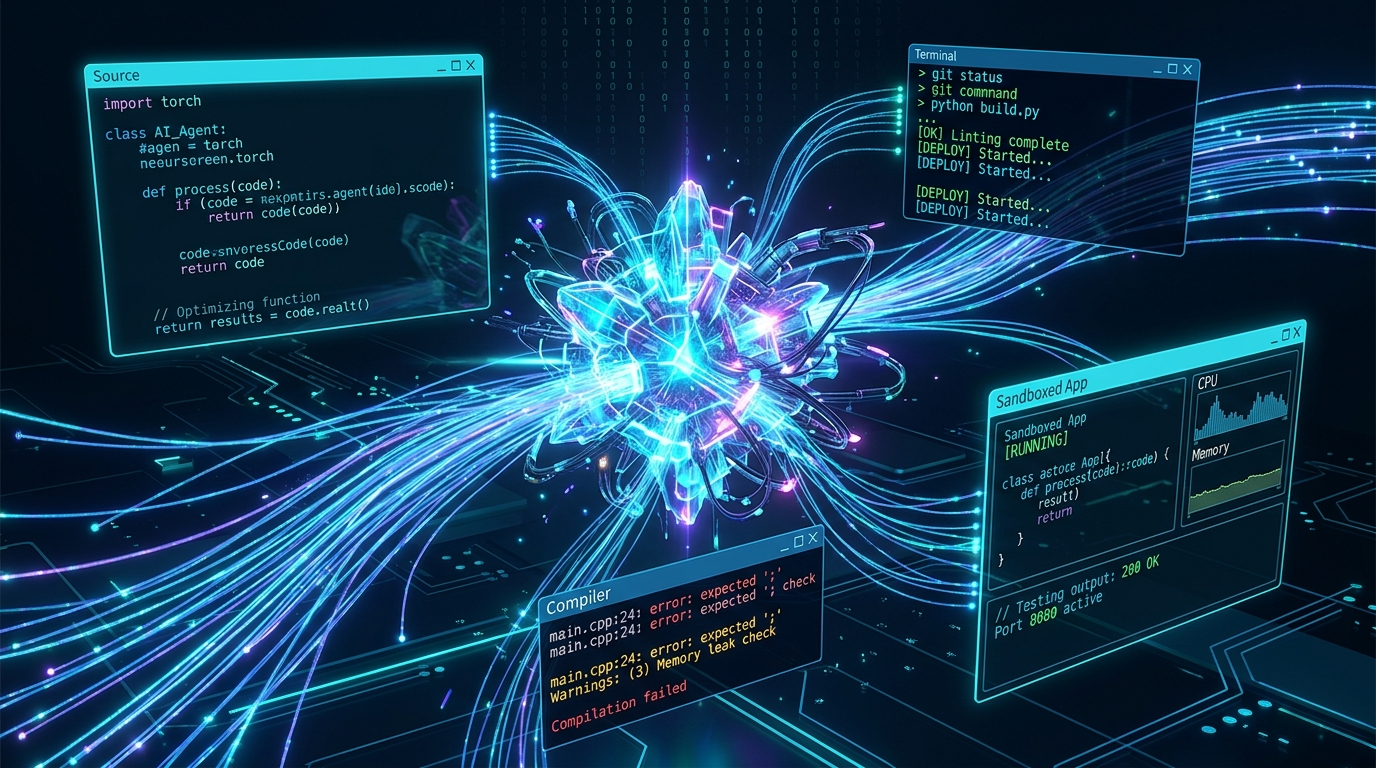
\includegraphics[width=0.95\textwidth]{images/agent_architecture.jpg}
    \caption{The Antigravity Agent Architecture: Decoupling reasoning from user interfaces, integrating live terminal sandboxes, compiler feedback loops, and intelligent context routing.}
    \label{fig:agent_architecture}
\end{figure}

\section{The Architectural Triad of Antigravity}
Antigravity re-architects the software development environment into three interconnected components:

\begin{conceptbox}[The Cognitive Engine]
Unlike standard conversational agents that respond in single back-and-forth turns, Antigravity executes an internal \textbf{Plan-Act-Observe Loop}. The model analyzes your codebase, formulates a multi-step execution tree, invokes filesystem and shell tools, observes the stdout/stderr return values, and self-corrects until its objective is verified.
\end{conceptbox}

\begin{enumerate}
    \item \textbf{The Core Reasoning Runtime}: Backed by multimodal Gemini models with multi-million token context windows. It processes code, terminal logs, UI screenshots, and git trees simultaneously.
    \item \textbf{The Execution Sandbox}: An isolated process environment where the agent can run shell commands (\texttt{make}, \texttt{cargo test}, \texttt{docker build}) without endangering your host OS or accessing unapproved networks.
    \item \textbf{The Customization Engine}: A tiered system composed of \textbf{Rules}, \textbf{Skills}, \textbf{Hooks}, and \textbf{MCP Servers} that allow any repository to instill its own engineering culture into the agent.
\end{enumerate}

\section{The Four Operational Surfaces of Antigravity}
Antigravity delivers its intelligence across four distinct form-factors:

\begin{table}[htbp]
\centering
\caption{Comparative Matrix: The Four Antigravity Surfaces}
\begin{tabularx}{\textwidth}{lXXXX}
\toprule
\textbf{Dimension} & \textbf{CLI (\texttt{agy})} & \textbf{Antigravity IDE} & \textbf{Antigravity 2.0} & \textbf{Python SDK} \\
\midrule
\textbf{Form Factor} & Terminal TUI & VS Code Fork & Electron Desktop & Python Library \\
\textbf{Ideal User} & DevOps, SREs, CLI ninjas & Full-stack Developers & Tech Leads, Architects & Automation Engineers \\
\textbf{Modality} & Turn-based & Tab, Inline, Chat & Canvas \& Artifacts & Headless Event Streams \\
\textbf{Host Footprint} & Minimal ($<$ 50MB) & Moderate (350MB) & Moderate (400MB) & Embedded in Python \\
\textbf{Interactive?} & Yes (REPL) & Yes (In-editor) & Yes (Multi-pane) & Programmatic (Async) \\
\textbf{Scriptable?} & Yes (Flags) & No (GUI focused) & No (GUI focused) & Completely (Pipelines) \\
\bottomrule
\end{tabularx}
\end{table}

---

\chapter{First Contact: Setup, CLI \& Configuration}

\section{System Prerequisites \& Installation}
Antigravity runs natively on modern 64-bit platforms: Linux (x86\_64 / ARM64), macOS (Apple Silicon / Intel), and Windows (via WSL2).

To install the Antigravity Command Line Interface (\texttt{agy}):
\begin{lstlisting}[language=bash, caption={Installing and verifying the Antigravity CLI}]
# Verify system environment
uname -m

# Install Antigravity CLI via standard package channel
curl -fsSL https://antigravity.google/install.sh | bash

# Verify installation
agy --version
\end{lstlisting}

\section{Authentication and Workspaces}
On your first run of \texttt{agy}, the runtime initiates an OAuth device-authorization flow. A secure browser tab opens, allowing you to link your Google Cloud or Vertex AI developer identity.

Once authenticated, your runtime secrets and tokens are encrypted under:
\begin{itemize}
    \item Linux/macOS: \texttt{\textasciitilde/.gemini/antigravity-cli/}
    \item Global Configuration: \texttt{\textasciitilde/.gemini/config/}
\end{itemize}

\begin{lstlisting}[language=bash, caption={Launching your first agent session}]
# Launch interactive REPL in current directory
cd ~/projects/my-microservice
agy

# Or launch directly with an initial instruction
agy "Review open git diff and run unit tests"
\end{lstlisting}

\section{Mastering CLI Flags and Headless Scripting}
The CLI provides powerful flags for scriptability and continuous integration:
\begin{itemize}
    \item \texttt{agy -w /path/to/project}: Explicitly specifies the working workspace root.
    \item \texttt{agy --model gemini-3.8-pro}: Overrides the active reasoning model.
    \item \texttt{agy --sandbox=strict}: Forces all bash tools to run inside an ephemeral sandbox container.
    \item \texttt{agy --approval=never}: Runs the agent fully autonomously (ideal for headless CI/CD runners).
    \item \texttt{agy --format=json}: Emits machine-parseable JSON streams of tool calls and output events.
\end{itemize}

\begin{labbox}[Project 1: WeatherCraft - CLI Bootstrapping]
Let us walk through using \texttt{agy} in the terminal to initialize a full-stack project from scratch without writing boilerplate manually:
\begin{lstlisting}[language=bash]
# In your terminal
mkdir weathercraft && cd weathercraft
agy "Initialize a FastAPI backend and a Next.js 14 frontend in ./backend and ./frontend. Configure CORS between localhost:3000 and 8000, write a health check endpoint, and verify it with pytest."
\end{lstlisting}
The agent will create the virtual environment, write \texttt{main.py}, set up \texttt{requirements.txt}, run \texttt{pip install}, generate \texttt{test\_main.py}, and execute \texttt{pytest} inside the terminal sandbox to prove it works before returning control to you.
\end{labbox}

---

\chapter{The Three Faces of Antigravity}

Antigravity meets engineers across three complementary surfaces: the in-editor IDE, the standalone 2.0 Desktop canvas, and the terminal TUI.

\section{The Antigravity IDE: Three AI Modalities}
Built on top of the open VS Code core, the Antigravity IDE integrates agentic capabilities directly into your editing canvas across three distinct interaction levels:

\subsection{1. Passive: Antigravity Tab (Autocomplete \& Supercomplete)}
Operating at the single-keystroke layer, Tab Autocomplete predicts your next intent:
\begin{itemize}
    \item \textbf{Contextual Autocomplete}: Suggests tokens at the cursor based on adjacent open tabs, diagnostics, and recent terminal outputs.
    \item \textbf{Supercomplete}: Generates multi-line diffs (including deletions and structural refactors) rendered in floating preview overlays.
    \item \textbf{Tab-to-Jump}: Predicts where your cursor needs to navigate next (e.g., jumping from a function definition to its unit test assertion) and teleports your cursor with a single \texttt{<Tab>}.
    \item \textbf{Tab-to-Import}: Automatically resolves missing symbols and injects import statements at the top of the file.
\end{itemize}

\subsection{2. Instructive: Inline Command (\texttt{Ctrl+I} / \texttt{Cmd+I})}
When you want targeted changes without switching focus to a chat window:
\begin{enumerate}
    \item Highlight a block of code (e.g., a messy SQL query or an unoptimized regex).
    \item Press \texttt{Ctrl+I} (or \texttt{Cmd+I} on macOS).
    \item Type: \textit{"Refactor this into parameterized sqlx query with error logging"}.
    \item Review the localized red/green diff right in your editor buffer and press \texttt{Enter} to accept.
\end{enumerate}

\subsection{3. Collaborative: Sidebar Chat \& Full Agent Mode}
When a task spans across files, requires terminal execution, or needs architectural deliberation, press \texttt{Ctrl+Shift+L} to engage the Sidebar Agent. The agent can read files, write new modules, execute \texttt{npm test}, diagnose failures, and consult online documentation.

\section{Antigravity 2.0: The Desktop Command Center}
Antigravity 2.0 is a standalone Electron desktop application tailored for high-autonomy multi-agent orchestration. It decouples agent execution from your text editor:

\begin{itemize}
    \item \textbf{Left-Hand Sidebar}: Manage multiple project workspaces, active background cron schedules, installed skills, and global security policies.
    \item \textbf{Chat Canvas}: Supports deep markdown artifacts, interactive review modals, and media uploads.
    \item \textbf{Auxiliary Telemetry Pane}: A multi-tab inspector showing live Subagent swarms, running background daemon logs, generated Artifact documents, and attached terminal sessions.
\end{itemize}

\section{Deep Dive: CLI vs IDE vs SDK in Real Engineering}
\begin{probox}[When to use which surface?]
Use the **IDE** when you are actively writing code, navigating files, and need inline diffs and autocomplete. Use the **CLI (\texttt{agy})** when you are logged into remote cloud VMs, managing servers over SSH, or chaining shell pipes. Use the **Desktop 2.0 Canvas** when conducting architectural redesigns, planning complex initiatives, or monitoring multiple background subagents. Use the **Python SDK** when embedding agent intelligence into CI/CD pipelines, Slack bots, or automated test runners.
\end{probox}

% =============================================================================
% PART II: CORE AGENTIC WORKFLOWS & PAIR PROGRAMMING
% =============================================================================
\part{Core Agentic Workflows \& Pair Programming (Intermediate)}

\chapter{The Art of Planning, Goal Architecture \& Review Loops}

\section{Why Unplanned Agents Fail}
The most common rookie mistake with AI coding assistants is issuing massive, ambiguous prompts:
\begin{quote}
\textit{"Rewrite my monolithic express app to clean architecture with TypeScript and add Docker."}
\end{quote}
An unplanned agent immediately begins hacking files. By step 14, it has broken TypeScript compilation. By step 25, it is deleting code to silence compiler errors. By step 40, your git working tree is ruined.

Antigravity solves this with formal \textbf{Planning Mode}.

\begin{probox}[The Planning Golden Rule]
Never let an agent touch code on a multi-file task until it has produced a formal \texttt{implementation\_plan.md} artifact and received your explicit sign-off.
\end{probox}

\section{The Anatomy of Planning Mode}
When confronted with architectural tasks, Antigravity enters Planning Mode:
\begin{enumerate}
    \item \textbf{Discovery \& Research}: The agent searches the project using read-only tools (\texttt{grep\_search}, \texttt{view\_file}, \texttt{list\_dir}). It inspects configuration files, existing test conventions, and database schemas.
    \item \textbf{Implementation Plan Artifact}: The agent drafts a comprehensive technical plan at \texttt{brain/<id>/implementation\_plan.md}.
    \item \textbf{User Review Gate}: The agent halts execution and presents an interactive review card. You can request changes or approve the plan with a click.
    \item \textbf{Execution \& Verification}: Once approved, the agent executes edits incrementally, running build commands at each stage.
    \item \textbf{Walkthrough Artifact}: Upon completion, the agent creates \texttt{walkthrough.md}, documenting every change made and providing proof of verification tests.
\end{enumerate}

\section{The Anatomy of an Unbreakable Goal Definition}
When running agents autonomously using the \texttt{/goal} command, the primary cause of runaway compute or degradation is \textbf{unbounded goal ambiguity}. If an agent does not have a mathematically deterministic stopping condition, it will hallucinate micro-optimizations indefinitely.

To prevent this, production Antigravity engineers use the \textbf{ATDG Framework (Acceptance Test-Driven Goal)}:

\begin{conceptbox}[The Four Pillars of an ATDG Goal]
Every autonomous goal statement must define:
\begin{enumerate}
    \item \textbf{The Invariant}: What existing behavior or contract must NOT change under any circumstance.
    \item \textbf{The Blast Radius}: The exact subdirectories or files that are mutable (everything else is read-only).
    \item \textbf{The Deterministic Oracle}: The exact terminal command that evaluates success (must return exit code 0).
    \item \textbf{The Stopping Rule}: The explicit condition under which the agent must stop and declare victory.
\end{enumerate}
\end{conceptbox}

\subsection{Vague Goal vs. Production-Grade ATDG Goal}
Compare the two following goal formulations:

\begin{promptbox}[Vague Goal (Fails 80\% of the time)]
\texttt{/goal Fix the broken checkout tests and make sure the API is robust.}
\end{promptbox}

\begin{promptbox}[ATDG Production Goal (Succeeds 99\% of the time)]
\texttt{/goal Invariant: Do NOT modify existing database schemas in prisma/schema.prisma or change the public response payload of POST /api/checkout.}\\
\textbf{Scope}: You are only permitted to edit files under \texttt{src/services/checkout/} and \texttt{src/utils/pricing.ts}.\\
\textbf{Oracle}: Run \texttt{'npm test test/checkout.spec.ts'}.\\
\textbf{Termination}: When all 14 tests pass with exit code 0 and \texttt{'npm run lint'} yields zero errors, stop and generate \texttt{walkthrough.md}.
\end{promptbox}

\section{The \texttt{/grill-me} Protocol}
If you know \textit{what} feature you want but haven't settled on the edge cases, invoke the \texttt{/grill-me} slash command. 

Instead of jumping into code, Antigravity assumes the role of a meticulous Principal Architect:
\begin{itemize}
    \item \textit{"How should we handle database connection timeouts during token refresh?"}
    \item \textit{"Should we invalidate all active user sessions upon password reset, or only the current device?"}
    \item \textit{"Do you want this API endpoint to be rate-limited by IP or by authenticated user ID?"}
\end{itemize}
Only once all design ambiguities are resolved does it formulate the plan.

\begin{labbox}[Project 2: AuthSentinel - Refactoring Legacy Auth in Planning Mode]
In this project, we refactor an insecure session-cookie service into an audited JWT architecture with rotating refresh tokens stored in Redis:
\begin{enumerate}
    \item Open the project in Antigravity IDE and type \texttt{/grill-me} in Sidebar Chat: \textit{"Refactor auth from memory sessions to Redis JWT with refresh token rotation."}
    \item The agent interviews you on secret rotation windows and cookie security flags (\texttt{HttpOnly}, \texttt{SameSite=Strict}).
    \item The agent generates \texttt{implementation\_plan.md} outlining the exact modifications across \texttt{auth.service.ts}, \texttt{redis.client.ts}, and \texttt{auth.guard.ts}.
    \item You review and approve the plan. The agent updates dependencies via \texttt{npm install}, writes the files, and launches \texttt{npm test} to verify that all 18 security regression tests pass.
\end{enumerate}
\end{labbox}

---

\chapter{Precision Context Engineering \& Battle-Tested Prompts}

\section{The Context Economy}
Modern LLMs boast massive context windows, but context is not free:
\begin{enumerate}
    \item \textbf{Latency}: Processing a 500,000-token prompt takes noticeably longer than a targeted 10,000-token prompt.
    \item \textbf{Attention Dilution}: When irrelevant files clutter the context window, the model's ability to notice critical subtleties in core logic degrades.
\end{enumerate}

\section{The Power of \texttt{@} Mentions}
Antigravity gives you surgical control over context using the \texttt{@} mention system:

\begin{table}[htbp]
\centering
\caption{Context Mention Resolvers in Antigravity}
\begin{tabularx}{\textwidth}{lX}
\toprule
\textbf{Mention Syntax} & \textbf{Resolved Context Injected} \\
\midrule
\texttt{@file:src/auth.ts} & Injects the full text of \texttt{src/auth.ts} into the turn. \\
\texttt{@folder:src/controllers/} & Injects directory listing and file summaries for that folder. \\
\texttt{@symbol:UserService} & Locates and injects the AST definition of the class or interface. \\
\texttt{@commit:HEAD\textasciitilde1} & Injects the git diff and commit log of the specified revision. \\
\texttt{@transcript:0e58b2} & Injects key context from an earlier conversation session. \\
\texttt{@mcp:github/search\_issues} & Injects schema and tool instructions for an MCP tool. \\
\bottomrule
\end{tabularx}
\end{table}

\section{The Production Prompt Engineering Taxonomy}
Prompting an autonomous agent is fundamentally different from prompting a conversational chatbot. An agent executes real tools. Below are four battle-tested production prompt patterns:

\subsection{1. The Zero-Regression Refactoring Blueprint}
When refactoring critical business logic, you must forbid interface breakage and speculative deletions:

\begin{promptbox}[Zero-Regression Refactoring]
You are refactoring \texttt{@file:src/services/billing.py} to use \texttt{async/await} with \texttt{httpx} instead of \texttt{requests}.\\
\textbf{Strict Invariants}:
\begin{enumerate}
    \item Preserve all public method signatures, argument names, and return type hints.
    \item Preserve all existing docstrings and inline business comments.
    \item Do NOT delete existing helper methods; mark them \texttt{@deprecated} if replaced.
    \item Run \texttt{'pytest tests/test\_billing.py'} before and after edits. All 22 tests must remain green.
\end{enumerate}
\end{promptbox}

\subsection{2. The Forensic Bug Triage Blueprint}
When diagnosing production errors, force the agent to reproduce the bug with a test \textit{before} writing a fix:

\begin{promptbox}[Forensic Triage Protocol]
Investigate error log \texttt{@file:logs/sentry\_event\_9402.json}.\\
Follow this mandatory 3-step triage loop:
\begin{enumerate}
    \item \textbf{Step 1 (Reproduction)}: Write a reproduction unit test in \texttt{tests/repro\_bug\_9402.py} that asserts the expected behavior and currently FAILS. Run \texttt{pytest} to demonstrate the failure.
    \item \textbf{Step 2 (Root-Cause Isolation)}: Inspect \texttt{@symbol:calculate\_rebate} and explain the exact mathematical flaw.
    \item \textbf{Step 3 (Remediation)}: Implement the minimal fix in \texttt{src/rebate.py}. Verify that \texttt{tests/repro\_bug\_9402.py} now passes and no existing tests regress.
\end{enumerate}
\end{promptbox}

\subsection{3. Negative Constraints Formulation}
Negative constraints prevent common LLM degradation behaviors:
\begin{itemize}
    \item \textbf{Anti-Mocking}: \textit{"Do NOT mock the database in integration tests; use the local testcontainers Postgres instance."}
    \item \textbf{Anti-Stubbing}: \textit{"Never leave \texttt{// TODO: implement later} stubs or placeholder functions. Every branch must be fully implemented."}
    \item \textbf{Scope Jail}: \textit{"Do NOT create files outside \texttt{src/features/search/}. Do NOT modify \texttt{package.json} without asking."}
\end{itemize}

\begin{warstory}[The Million-Token Hallucination Trap]
A development team once attached their entire 2GB \texttt{node\_modules} folder to an agent prompt via a misplaced wildcard. The agent spent 12 minutes digesting 800,000 tokens of minified JavaScript, completely missed the two-line syntax bug in the user's controller, and timed out. By switching to \texttt{@symbol:UserController} and \texttt{@file:src/routes.ts}, the context dropped to 1,400 tokens, and the bug was fixed in 4 seconds.
\end{warstory}

---

\chapter{The Iron Sandbox: Security \& Permissions}

\begin{cautionbox}[The Threat Model of Autonomous Agents]
An agent capable of executing terminal commands can accidentally run \texttt{rm -rf /}, leak environment secrets to public pastebins, or download malicious dependencies. Security must be enforced at the runtime level, not left to model obedience.
\end{cautionbox}

\section{Execution Policies}
Antigravity enforces configurable permission levels:
\begin{itemize}
    \item \textbf{\texttt{strict}}: The agent must request interactive user approval before running any command, reading unapproved files, or touching the network.
    \item \textbf{\texttt{request-review}}: Read operations proceed automatically; write operations and shell commands require user approval.
    \item \textbf{\texttt{proceed-in-sandbox}}: The agent executes commands freely, but strictly inside an unprivileged Linux container sandbox with isolated namespaces.
    \item \textbf{\texttt{always-proceed}}: Zero confirmation prompts. Intended exclusively for isolated VM sandboxes or test runners.
\end{itemize}

\section{Project-Level Allow and Deny Lists}
Configure security controls in \texttt{.agents/settings.json}:
\begin{lstlisting}[caption={Hardening Antigravity security policies}]
{
  "security": {
    "terminalSandbox": true,
    "nonWorkspaceAccess": "deny",
    "internetAccess": "allow",
    "commandAllowlist": [
      "git *",
      "npm test*",
      "cargo check",
      "go test ./**"
    ],
    "commandDenylist": [
      "rm -rf *",
      "curl * | bash",
      "sudo *",
      "dd *"
    ]
  }
}
\end{lstlisting}

% =============================================================================
% PART III: THE CUSTOMIZATION ENGINE
% =============================================================================
\part{The Customization Engine (Advanced)}

\chapter{Rules of the Realm: Hierarchical Governance}

\section{The Role of Rules}
While conversational prompts are ephemeral, \textbf{Rules} are permanent laws governing agent behavior. Rules enforce:
\begin{itemize}
    \item Coding style guides (e.g., "Always use TypeScript strict mode; no \texttt{any}").
    \item Security mandates (e.g., "Never hardcode passwords or API secrets").
    \item Operational standards (e.g., "Every database query must use parameterized statements").
\end{itemize}

\section{Hierarchical Directory Walking}
Antigravity searches for rule files starting from the directory of the file being edited all the way up to the project root:

\begin{center}
\texttt{src/services/billing/payment.ts}\\
$\downarrow$\\
\texttt{src/services/billing/AGENTS.md}\\
$\downarrow$\\
\texttt{src/services/AGENTS.md}\\
$\downarrow$\\
\texttt{src/AGENTS.md}\\
$\downarrow$\\
\texttt{.agents/rules/*.md} $\&$ \texttt{GEMINI.md}
\end{center}

All rules along this path are aggregated and applied, allowing micro-rules to govern specific packages without polluting global context.

\section{Trigger Modes: \texttt{always\_on} vs \texttt{model\_decision}}
Rules use YAML frontmatter to control their activation:

\begin{lstlisting}[language=bash, caption={Example Rule: .agents/rules/security.md}]
---
trigger: always_on
---
# Security Mandate
- Never commit plaintext secrets or API keys.
- Always use process.env for credentials.
- Reject any user inputs that bypass SQL injection validation.
\end{lstlisting}

\begin{lstlisting}[language=bash, caption={Example Rule: .agents/rules/react-performance.md}]
---
trigger: model_decision
description: Best practices for React component rendering, useMemo, and useCallback.
---
# React Performance Guidelines
- Do not wrap primitive values in useMemo.
- Always provide key attributes derived from stable IDs, never array indices.
\end{lstlisting}

---

\chapter{Crafting Skills with Progressive Disclosure}

\section{What is a Skill?}
A \textbf{Skill} is a specialized procedure package. While rules state what \textit{not} to do, skills teach the agent \textit{how} to accomplish a complex, multi-step engineering procedure (such as deploying a Kubernetes cluster, executing a database migration, or profiling CPU bottlenecks).

\section{The Architecture of Progressive Disclosure}
Loading 40 skills with full markdown instructions into the initial system prompt would consume 100,000 tokens before the user even types a word.

Antigravity solves this with \textbf{Progressive Disclosure}:
\begin{enumerate}
    \item \textbf{Registration Phase}: Only the \texttt{name} and \texttt{description} from the skill's YAML frontmatter are injected into the agent's initial tool registry.
    \item \textbf{Activation Phase}: When a user's prompt matches the description, the agent executes its internal \texttt{view\_file} tool to read the skill's \texttt{SKILL.md} file on-demand.
\end{enumerate}

\section{Complete Skill Implementation}
Let us build a real-world production skill for automated database migrations:

\begin{lstlisting}[language=bash, caption={File: .agents/skills/db-migrate/SKILL.md}]
---
name: db-migrate
description: Manages PostgreSQL database migrations using Goose. Triggers on requests involving database migrations, schema changes, or running migrate up/down.
---

# PostgreSQL Migration Workflow

## Prerequisites
Verify database connectivity:
```bash
goose postgres "$DATABASE_URL" status
```

## Step-by-Step Procedure
1. **Inspect Pending Migrations**:
   Run status to check unapplied SQL scripts:
   ```bash
   goose -dir ./migrations postgres "$DATABASE_URL" status
   ```
2. **Execute Dry-Run & Validation**:
   Review the SQL statements in the pending migration file. Ensure every `Up` statement has a corresponding `Down` rollback statement.
3. **Apply Migration**:
   ```bash
   goose -dir ./migrations postgres "$DATABASE_URL" up
   ```
4. **Verify Table Schema**:
   Verify the schema changes using psql:
   ```bash
   psql "$DATABASE_URL" -c "\d+ users"
   ```
\end{lstlisting}

\begin{labbox}[Project 3: CloudScale - Authoring Enterprise Skills and MCP]
In this project, we package an internal release automation skill that validates container images against Trivy vulnerability scanners, deploys to staging via Helm, runs integration smoke tests, and updates the Jira release ticket via MCP tools.
\end{labbox}

---

\chapter{Deterministic Gates with Hooks}

\begin{conceptbox}[Probabilistic vs. Deterministic Guardrails]
A prompt or rule is \textit{probabilistic}: the LLM tries to follow it, but there is always a non-zero chance of a mistake. A \textbf{Hook} is \textit{deterministic}: it is a shell script executed by the operating system before or after a tool call. If the hook fails, the action is stopped dead in its tracks.
\end{conceptbox}

\section{Configuring \texttt{hooks.json}}
Hooks are configured in \texttt{.agents/hooks.json}:

\begin{lstlisting}[caption={Configuring lifecycle hooks in .agents/hooks.json}]
{
  "hooks": {
    "pre_tool_use": [
      {
        "matcher": { "tool": "run_command" },
        "command": "python3 .agents/hooks/validate_command.py",
        "blocking": true,
        "timeoutMs": 5000
      }
    ],
    "post_tool_use": [
      {
        "matcher": { "tool": "replace_file_content" },
        "command": "npx prettier --write \"$ANTIGRAVITY_MODIFIED_FILE\"",
        "blocking": false
      }
    ]
  }
}
\end{lstlisting}

\section{Writing a Blocking Pre-Tool Validation Hook}
Here is a Python script that prevents the agent from running destructive Git commands on protected branches:

\begin{lstlisting}[language=python, caption={File: .agents/hooks/enforce\_branch\_protection.py}]
import os
import sys
import json
import subprocess

# Read tool invocation details from environment
command_to_run = os.environ.get("ANTIGRAVITY_COMMAND_LINE", "")

# Check current git branch
branch = subprocess.check_output(
    ["git", "rev-parse", "--abbrev-ref", "HEAD"], 
    text=True
).strip()

if branch in ["main", "master", "production"]:
    if "push" in command_to_run or "reset --hard" in command_to_run:
        sys.stderr.write(
            f"ERROR: Destructive command blocked on protected branch '{branch}'!\n"
        )
        sys.exit(1) # Non-zero exit code halts tool execution

sys.exit(0)
\end{lstlisting}

---

\chapter{Model Context Protocol (MCP) Integration}

\section{What is MCP?}
The \textbf{Model Context Protocol (MCP)} is an open, standardized protocol created to connect AI agents with external data stores, SaaS APIs, and custom tooling over JSON-RPC (via standard I/O or SSE).

Through MCP, Antigravity can directly:
\begin{itemize}
    \item Query production SQL databases.
    \item Inspect and review GitHub Pull Requests and Issues.
    \item Fetch CloudWatch or Datadog telemetry logs.
    \item Trigger AWS Lambda or Google Cloud Run deployments.
\end{itemize}

\section{Configuring \texttt{mcp\_config.json}}
Add server definitions to \texttt{.agents/mcp\_config.json}:

\begin{lstlisting}[caption={Connecting external tools via MCP}]
{
  "mcpServers": {
    "github": {
      "command": "npx",
      "args": ["-y", "@modelcontextprotocol/server-github"],
      "env": {
        "GITHUB_PERSONAL_ACCESS_TOKEN": "ghp_secureToken12345"
      }
    },
    "production_postgres": {
      "command": "docker",
      "args": [
        "run", "-i", "--rm",
        "-e", "DATABASE_URL=postgres://readonly@db.internal:5432/prod",
        "mcp/postgres"
      ]
    }
  }
}
\end{lstlisting}

\section{Lazy vs. Eager Tool Loading}
Connecting 10 MCP servers could easily register 300+ tools. If all 300 tool definitions were injected into the system prompt, context overhead would be immense.

Antigravity handles this by classifying MCP tools as \textbf{Lazy Loaded}:
\begin{itemize}
    \item The agent is provided a meta-tool: \texttt{call\_mcp\_tool(server, tool, args)}.
    \item It reads the tool's JSON schema only when it decides to call it, keeping the primary prompt lean.
\end{itemize}

% =============================================================================
% PART IV: PROGRAMMATIC AGENT MASTERY & THE SKILL STACK
% =============================================================================
\part{Programmatic Agent Mastery \& The Skill Stack (Expert)}

\chapter{The Antigravity Python SDK}

\section{Headless Agent Orchestration}
While the IDE and CLI cater to humans sitting at keyboards, the modern enterprise requires \textbf{headless agent pipelines}: automated PR reviewers, nightly security patchers, and autonomous triage bots.

Google provides the official Python SDK:
\begin{lstlisting}[language=bash, caption={Installing the Python SDK}]
pip install google-antigravity
\end{lstlisting}

\begin{figure}[htbp]
    \centering
    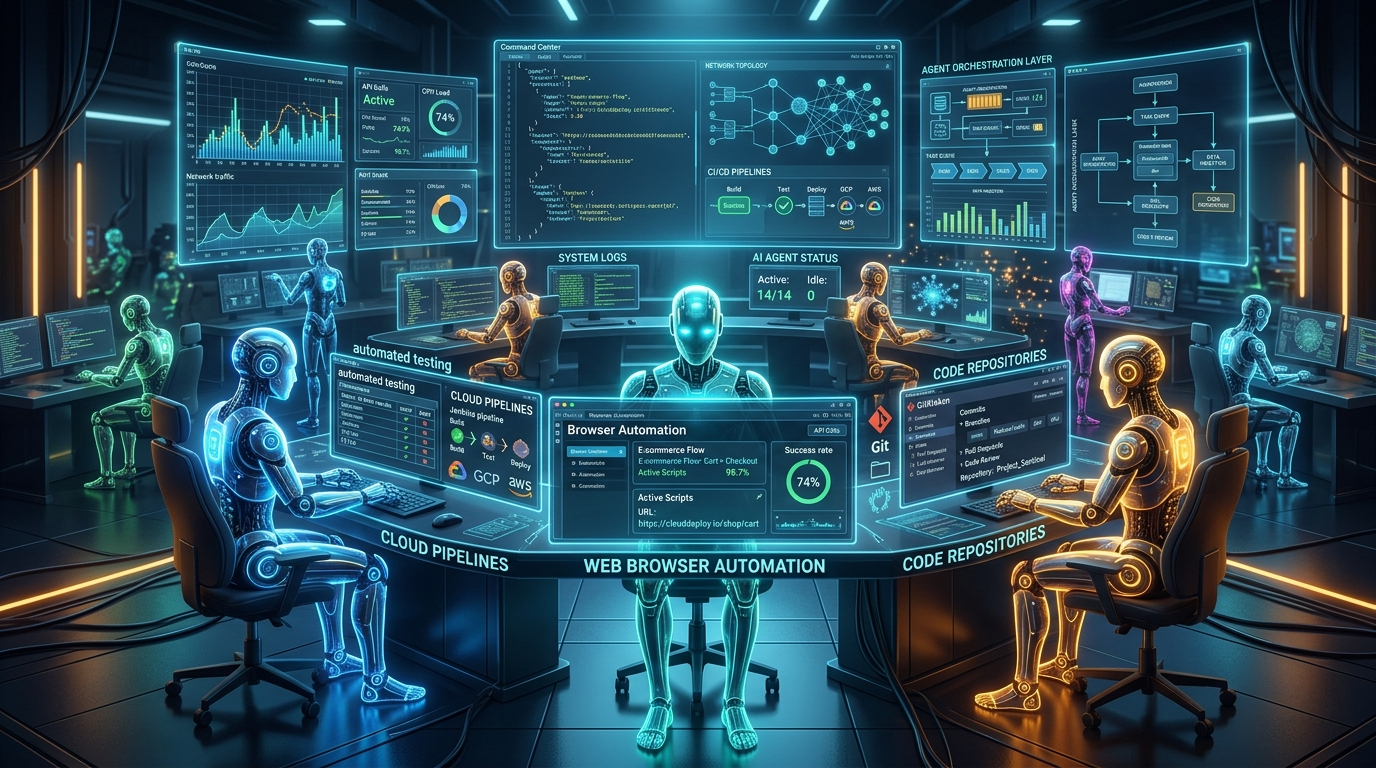
\includegraphics[width=0.95\textwidth]{images/multi_agent_swarm.jpg}
    \caption{Multi-Agent Swarm Orchestration: Spawning autonomous subagents for automated testing, cloud pipelines, and browser automation.}
    \label{fig:multi_agent_swarm}
\end{figure}

\section{Building an Asynchronous SRE Agent}
Below is a complete, production-ready Python script using the SDK:

\begin{lstlisting}[language=python, caption={Automated SRE Diagnostic Bot with google-antigravity}]
import asyncio
import sys
from google.antigravity import (
    Agent, 
    LocalAgentConfig, 
    CapabilitiesConfig, 
    SecurityPolicy
)

async def run_diagnostics():
    # Configure the programmatic agent
    config = LocalAgentConfig(
        workspace_dir="/var/www/ecommerce-core",
        system_instructions=(
            "You are an expert Site Reliability Engineer. "
            "Inspect recent crash logs, locate the bug in source code, "
            "and create a pull request with unit test coverage."
        ),
        capabilities=CapabilitiesConfig(
            allow_file_modifications=True,
            allow_terminal_execution=True,
            allow_internet_access=True
        ),
        security_policy=SecurityPolicy(
            terminal_sandbox=True,
            non_workspace_access="deny"
        )
    )

    # Agent acts as an async context manager
    async with Agent(config) as agent:
        print("[+] Agent session established. Dispatching mission...")
        
        response = await agent.chat(
            "Diagnose 500 errors reported in /var/log/app.err.log"
        )

        # Stream internal chain-of-thought reasoning
        async for thought in response.thoughts:
            print(f"[THOUGHT] {thought}")

        # Intercept and log tool calls
        async for tool_call in response.tool_calls:
            print(f"[TOOL] Invoking {tool_call.name} with {tool_call.args}")

        # Stream final conversational tokens
        print("\n--- Final Agent Report ---")
        async for token in response:
            sys.stdout.write(token)
            sys.stdout.flush()
        print()

if __name__ == "__main__":
    asyncio.run(run_diagnostics())
\end{lstlisting}

\section{Deep Architectural Comparison: CLI vs. SDK}
Understanding the boundary between \texttt{agy} and \texttt{google-antigravity}:
\begin{itemize}
    \item \textbf{The CLI (\texttt{agy})}: Designed for interactive human sessions or one-shot command lines. The output is rendered via a terminal UI (Rich/TUI). Error handling stops and asks the user for guidance.
    \item \textbf{The Python SDK}: Designed for programmatic integration into larger distributed systems. Yields strongly-typed async events (\texttt{ThoughtDelta}, \texttt{ToolCallEvent}, \texttt{StreamChunk}). Gives the host Python process complete programmatic control to intercept tool calls, inject synthetic results, or route tasks to worker queues.
\end{itemize}

---

\chapter{Swarms, Browser Agents \& Daemons}

\section{Subagent Delegation (\texttt{invoke\_subagent})}
When a task is too vast for a single context window, the primary agent can spawn specialized \textbf{Subagents}:

\begin{itemize}
    \item \textbf{Context Isolation}: The subagent begins with a clean context, insulated from conversational noise in the main thread.
    \item \textbf{Specialized Personas}: Subagent A is spun up as a "Database Index Optimizer"; Subagent B is spun up as a "Frontend CSS Expert".
    \item \textbf{Return Value Consolidation}: When the subagent completes its task, it returns a concise summary back to the parent agent.
\end{itemize}

\section{Autonomous Browser Automation}
Testing web applications requires seeing what the user sees. Antigravity includes a dedicated browser automation subagent:
\begin{enumerate}
    \item Launches a headless Chromium instance.
    \item Navigates to local development URLs (e.g., \texttt{http://localhost:3000}).
    \item Types into form inputs, clicks buttons, and asserts DOM changes.
    \item \textbf{Automatic WebP Video Recording}: Automatically captures a recording of the entire browser session and embeds it in the walkthrough artifact so you can visually verify the UI test.
\end{enumerate}

\section{Background Daemons \& The Scheduler}
Rather than locking the terminal with \texttt{sleep 30}, Antigravity uses the \texttt{schedule} tool:
\begin{itemize}
    \item \textbf{One-Shot Timers}: Fires a notification after $N$ seconds, waking up the agent reactively.
    \item \textbf{Recurring Cron Jobs}: Configured with standard 5-field cron syntax (\texttt{*/30 * * * *}) to run automated health checks or polling jobs.
\end{itemize}

\begin{labbox}[Project 4: AutoSRE Sentinel - Building a 24/7 Monitoring Agent]
We create a standalone Python daemon using the Antigravity SDK:
\begin{enumerate}
    \item The script connects to an AWS SQS queue receiving alerts from Datadog.
    \item When an anomaly is detected, it spins up an \texttt{Agent} instance scoped to the offending microservice repo.
    \item The agent inspects recent git commits, reproduces the failure in a container sandbox, runs headless browser verification with video recording, commits a hotfix to a branch, and opens a GitHub Pull Request with the WebP video attached.
\end{enumerate}
\end{labbox}

---

\chapter{Enterprise Monorepos \& CI/CD}

\section{Scaling Antigravity in Large Repositories}
In monorepos containing millions of lines of code, global rules become unwieldy. Follow the \textbf{Domain-Partitioned Pattern}:

\begin{lstlisting}[language=bash, caption={Monorepo directory layout for Antigravity}]
monorepo-root/
|-- .agents/
|   |-- rules/
|   |   \-- global-security.md    # Applies across all services
|   \-- hooks.json
|-- services/
|   |-- payments/
|   |   |-- .agents/
|   |   |   \-- rules/
|   |   |       \-- pci-dss.md    # Strict financial compliance rules
|   |   \-- AGENTS.md
|   \-- search/
|       |-- .agents/
|       |   \-- rules/
|       |       \-- elastic.md    # Indexing guidelines
|       \-- AGENTS.md
\end{lstlisting}

\section{GitHub Actions CI/CD Integration}
Run Antigravity as an automated pull-request review bot:

\begin{lstlisting}[caption={File: .github/workflows/antigravity\_review.yml}]
name: Antigravity Autonomous PR Review
on:
  pull_request:
    types: [opened, synchronize]

jobs:
  agentic-review:
    runs-on: ubuntu-latest
    permissions:
      contents: write
      pull-requests: write
    steps:
      - name: Checkout Code
        uses: actions/checkout@v4
        with:
          fetch-depth: 0

      - name: Set up Python
        uses: actions/setup-python@v5
        with:
          python-version: '3.11'

      - name: Install Dependencies
        run: |
          pip install google-antigravity PyGithub

      - name: Run Antigravity Review Bot
        env:
          GEMINI_API_KEY: ${{ secrets.GEMINI_API_KEY }}
          GITHUB_TOKEN: ${{ secrets.GITHUB_TOKEN }}
        run: |
          python3 .agents/ci/review_pr.py
\end{lstlisting}

---

\chapter{The AI Developer's Skill Stack: Thriving in the Agentic Era}

\section{The Evolution: From Code Typist to Systems Director}
With the advent of autonomous coding agents, the economic value of memorizing programming syntax, library APIs, and boilerplate patterns has plummeted toward zero. Conversely, the value of \textbf{architectural decomposition, rigorous verification design, and systems-level orchestration} has grown exponentially.

The engineer of the future is not a typist: they are an \textbf{Executive Director of AI Engineering Swarms}.

\section{The Six Core Pillars of AI Engineering}

\begin{conceptbox}[The Six Pillars of the Modern AI Engineer]
To operate Antigravity at enterprise scale, engineers must develop mastery across six core dimensions:
\begin{enumerate}
    \item \textbf{Test Harness Architecture (The Oracle Problem)}: Constructing deterministic, fast, automated test suites that serve as the ground truth for agent verification.
    \item \textbf{Attention \& Context Curation}: Designing lean context boundaries, navigating AST symbol graphs, and eliminating prompt noise.
    \item \textbf{Governance Stratification}: Intuitively knowing whether an instruction belongs in a conversational prompt, a hierarchical rule, a progressive skill, or a deterministic hook.
    \item \textbf{Defensive Sandboxing \& Blast Radius Isolation}: Hardening execution environments, establishing read/write jails, and restricting network capabilities.
    \item \textbf{Agent Observability \& Log Forensics}: Analyzing chain-of-thought streams, parsing agent transcripts, and diagnosing tool execution faults.
    \item \textbf{Deconstructive Systems Decomposition}: Breaking complex product features into modular sub-tasks that can be leased to specialized subagents.
\end{enumerate}
\end{conceptbox}

\subsection{1. Solving the Oracle Problem}
An AI agent can only generate code as good as the test suite that evaluates it. If your codebase has no tests, an agent operating under \texttt{/goal} will consider its job done as soon as the syntax compiles—regardless of whether business logic is broken. AI engineers spend 60\% of their effort designing bulletproof test harnesses and property-based tests that act as objective truth oracles.

\subsection{2. The Tri-Layer Governance Stratum}
When establishing repository standards, use the following decision matrix:
\begin{itemize}
    \item \textbf{Use Prompts}: For ephemeral, one-time instructions specific to the immediate task.
    \item \textbf{Use Rules (\texttt{.agents/rules/})}: For universal coding style, lint standards, and architectural conventions that must apply across multiple turns.
    \item \textbf{Use Skills (\texttt{.agents/skills/})}: For complex multi-step procedures (runbooks, deployments, migrations) loaded on-demand via progressive disclosure.
    \item \textbf{Use Hooks (\texttt{hooks.json})}: For non-negotiable security gates (e.g., blocking commits to main, scanning secrets) that must NEVER be bypassed by LLM hallucination.
\end{itemize}

\chapter{Interfacing Antigravity: WhatsApp, Telegram \& Google Workspace}

\section{The Omnichannel Agent Architecture}
In modern engineering teams, problems do not wait for developers to open an IDE. Critical deployment failures happen during off-hours, executive queries require instant telemetry summaries, and on-call engineers triage alerts on mobile devices.

To meet engineers wherever they are, Antigravity supports an \textbf{Omnichannel Gateway Architecture}:

\begin{center}
\textbf{[WhatsApp / Telegram]} $\longleftrightarrow$ \textbf{[Gateway Controller]} $\longleftrightarrow$ \textbf{[Antigravity Python SDK]} $\longleftrightarrow$ \textbf{[Google Sheets / Gmail / Codebases]}
\end{center}

\begin{conceptbox}[The Gateway Decoupling Pattern]
Never connect conversational chat apps directly to raw bash toolkits without a mediating gateway. The Gateway Controller:
\begin{enumerate}
    \item \textbf{Maps User Identities}: Resolves a Telegram \texttt{chat\_id} or WhatsApp phone number to authorized repository permissions.
    \item \textbf{Buffers Async Streaming}: Aggregates agent token deltas into conversational messages and handles Telegram/WhatsApp rate limits.
    \item \textbf{Dispatches Artifacts}: Converts generated markdown reports, diff patches, or test videos into native mobile attachments.
\end{enumerate}
\end{conceptbox}

\section{WhatsApp Cloud API Integration Workflow}
The Meta WhatsApp Business Cloud API operates over webhooks. Below is the complete production workflow for an autonomous Antigravity WhatsApp bot:

\begin{figure}[htbp]
\centering
\begin{conceptbox}[Workflow: WhatsApp Inbound Triage]
1. \textbf{Inbound Message}: User sends: \textit{"Run smoke tests on staging and notify on-call"}.\\
2. \textbf{Webhook Receiver}: FastAPI validates the HMAC-SHA256 signature and parses the payload.\\
3. \textbf{Agent Execution}: The Antigravity Python SDK executes \texttt{pytest} inside the isolated sandbox.\\
4. \textbf{WhatsApp Response}: Formatted status and test summary are delivered back to the WhatsApp chat.
\end{conceptbox}
\end{figure}

\subsection{Production WhatsApp Gateway Server}
\begin{lstlisting}[language=python, caption={FastAPI WhatsApp Gateway for Antigravity}]
import os
import httpx
from fastapi import FastAPI, Request, Query, Response
from google.antigravity import Agent, LocalAgentConfig, CapabilitiesConfig

app = FastAPI()

WHATSAPP_TOKEN = os.environ["WHATSAPP_API_TOKEN"]
PHONE_NUMBER_ID = os.environ["WHATSAPP_PHONE_ID"]
VERIFY_TOKEN = os.environ["WHATSAPP_VERIFY_TOKEN"]

# 1. Verification Challenge (Meta Setup)
@app.get("/webhook")
async def verify_webhook(
    mode: str = Query(..., alias="hub.mode"),
    token: str = Query(..., alias="hub.verify_token"),
    challenge: str = Query(..., alias="hub.challenge")
):
    if mode == "subscribe" and token == VERIFY_TOKEN:
        return Response(content=challenge, media_type="text/plain")
    return Response(status_code=403)

# 2. Inbound Message Handler
@app.post("/webhook")
async def handle_whatsapp_message(request: Request):
    payload = await request.json()
    try:
        entry = payload["entry"][0]["changes"][0]["value"]
        messages = entry.get("messages", [])
        if not messages:
            return {"status": "ignored"}

        user_msg = messages[0]["text"]["body"]
        sender_phone = messages[0]["from"]

        # 3. Dispatch to Antigravity Agent
        config = LocalAgentConfig(
            workspace_dir="/var/www/ecommerce-api",
            capabilities=CapabilitiesConfig(allow_terminal_execution=True)
        )
        async with Agent(config) as agent:
            response = await agent.chat(user_msg)
            full_text = ""
            async for token in response:
                full_text += token

        # 4. Reply via WhatsApp Graph API
        url = f"https://graph.facebook.com/v20.0/{PHONE_NUMBER_ID}/messages"
        headers = {"Authorization": f"Bearer {WHATSAPP_TOKEN}"}
        body = {
            "messaging_product": "whatsapp",
            "to": sender_phone,
            "type": "text",
            "text": {"body": full_text[:4096]}
        }
        async with httpx.AsyncClient() as client:
            await client.post(url, json=body, headers=headers)

    except Exception as e:
        print(f"Error handling webhook: {e}")
    return {"status": "ok"}
\end{lstlisting}

\section{Telegram Bot Integration Workflow}
Telegram provides superior support for long messages, markdown formatting, document uploads, and dynamic message editing.

\subsection{Real-Time Thinking Stream over Telegram}
Using the \texttt{response.thoughts} stream from the Antigravity Python SDK, we can update a Telegram message in real-time as the agent ponders:

\begin{lstlisting}[language=python, caption={Telegram Bot with Real-Time Thinking Stream}]
import os
import asyncio
from telegram import Update
from telegram.ext import Application, CommandHandler, MessageHandler, filters, ContextTypes
from google.antigravity import Agent, LocalAgentConfig, CapabilitiesConfig

TELEGRAM_BOT_TOKEN = os.environ["TELEGRAM_BOT_TOKEN"]

async def handle_message(update: Update, context: ContextTypes.DEFAULT_TYPE):
    user_prompt = update.message.text
    status_msg = await update.message.reply_text("Thinking...")

    config = LocalAgentConfig(
        workspace_dir="/home/dev/microservices/payment-hub",
        capabilities=CapabilitiesConfig(allow_file_modifications=True, allow_terminal_execution=True)
    )

    async with Agent(config) as agent:
        response = await agent.chat(user_prompt)

        # Stream thoughts to Telegram
        thought_accumulator = ""
        last_edit_time = asyncio.get_event_loop().time()

        async for thought in response.thoughts:
            thought_accumulator += thought
            now = asyncio.get_event_loop().time()
            # Throttle Telegram edits to prevent rate limits (max 1 edit / 1.5s)
            if now - last_edit_time > 1.5:
                preview = thought_accumulator[-200:].strip()
                await status_msg.edit_text(f"Working...\n\nThought: _{preview}_", parse_mode="Markdown")
                last_edit_time = now

        # Stream and accumulate final answer
        final_answer = ""
        async for token in response:
            final_answer += token

        # Deliver final message
        await status_msg.edit_text(final_answer[:4000])

def main():
    app = Application.builder().token(TELEGRAM_BOT_TOKEN).build()
    app.add_handler(MessageHandler(filters.TEXT & ~filters.COMMAND, handle_message))
    print("[*] Antigravity Telegram Bot polling...")
    app.run_polling()

if __name__ == "__main__":
    main()
\end{lstlisting}

\section{Google Workspace Integration (Sheets \& Gmail via MCP)}
Antigravity seamlessly interacts with Google Sheets and Gmail through the **Model Context Protocol (MCP)** or direct Google API integrations.

\subsection{1. Google Sheets as an Autonomous Audit Ledger}
Configure the Google Sheets MCP server in \texttt{.agents/mcp\_config.json}:

\begin{lstlisting}[caption={Connecting Google Sheets MCP Server}]
{
  "mcpServers": {
    "google_sheets": {
      "command": "npx",
      "args": ["-y", "@modelcontextprotocol/server-google-sheets"],
      "env": {
        "GOOGLE_SERVICE_ACCOUNT_KEY_PATH": "/secrets/google_service_account.json"
      }
    },
    "gmail": {
      "command": "npx",
      "args": ["-y", "@modelcontextprotocol/server-gmail"],
      "env": {
        "GMAIL_CREDENTIALS_PATH": "/secrets/gmail_oauth.json"
      }
    }
  }
}
\end{lstlisting}

\subsection{2. Automated Bug Ledger \& Executive Email Workflow}
With Google Workspace MCP tools registered, an agent can execute multi-step cross-platform workflows:

\begin{promptbox}[Multi-Platform Orchestration Prompt]
Investigate failing payment webhook in \texttt{@file:logs/webhook\_errors.log}.
\begin{enumerate}
    \item Fix the bug in \texttt{src/webhooks/stripe.ts} and verify with \texttt{'npm test'}.
    \item Append a new audit row to Google Sheet \texttt{'Production Incident Log'} with timestamp, error summary, file changed, and author.
    \item Draft an email in Gmail to \texttt{'engineering-leads@company.com'} with subject \texttt{'[INCIDENT RESOLVED] Stripe Webhook Fix'} detailing the root cause and PR link.
\end{enumerate}
\end{promptbox}

\begin{labbox}[Project 5: The Omnichannel SRE Concierge]
An on-call engineer receives an alert on \textbf{WhatsApp} while commuting. They reply: \textit{"@antigravity investigate high CPU on order service and post incident summary to Sheets"}.
\begin{enumerate}
    \item The WhatsApp Gateway routes the prompt to the Antigravity agent.
    \item The agent inspects container stats, identifies a runaway regex in \texttt{validator.py}, writes an optimized replacement, and runs the test suite.
    \item The agent appends a structured log row to the shared team \textbf{Google Sheet}.
    \item The agent drafts a post-mortem email in \textbf{Gmail} for the team.
    \item The agent sends a \textbf{Telegram} message to the team channel with the git diff and sends a confirmation to the engineer on \textbf{WhatsApp} with the resolution status.
\end{enumerate}
\end{labbox}

% =============================================================================
% CHAPTER 16: CLOUD DEPLOYMENT & HOSTING PLATFORMS
% =============================================================================
\chapter{Cloud Deployment, Production Architectures \& Hosting Platforms}

\section{The Paradigm Shift: From Local Pair to Cloud-Native Autonomous Agent}
While running Antigravity inside a local IDE provides immense productivity for day-to-day coding, the true power of autonomous agentic systems is unlocked when they operate continuously in the cloud. Cloud-deployed agents function as autonomous site reliability engineers, 24/7 background security auditors, omnichannel triage bots, and persistent PR reviewers.

Operating in production requires decoupling the agent's \textbf{execution runtime} from the \textbf{state store}:

\begin{center}
\textbf{[Inbound Events (Webhooks/Queues)]} $\longrightarrow$ \textbf{[Stateless Container Cluster (Cloud Run/Fly/Railway)]} $\longleftrightarrow$ \textbf{[Persistent Brain Store (EFS/GCS/NVMe)]}
\end{center}

\begin{conceptbox}[Stateful Brain vs. Stateless Compute]
Antigravity stores conversation transcripts, plans, artifacts, and execution scratch files inside the Brain directory (\texttt{/var/data/antigravity/brain}). In ephemeral container environments (such as Cloud Run or AWS Fargate), containers can be restarted or scaled down at any moment. 
\begin{enumerate}
    \item \textbf{Ephemeral Sandboxes}: Scratch execution directories (\texttt{/tmp} and \texttt{workspace/}) should be treated as ephemeral and discarded after a session.
    \item \textbf{Durable Brain Persistence}: Mount a persistent cloud volume (GCP Cloud Storage FUSE, AWS EFS, or Fly.io Volume) to \texttt{ANTIGRAVITY\_DATA\_DIR} so agent memories and audit trails survive container recycling.
\end{enumerate}
\end{conceptbox}

\section{Containerizing Antigravity: The Hardened Production Dockerfile}
Deploying an AI agent capable of executing shell commands and running browser subagents requires a carefully hardened container environment:
\begin{enumerate}
    \item \textbf{Non-Root Security}: Never run the container daemon as \texttt{root}. Drop all capabilities (\texttt{--cap-drop=ALL}) and assign a dedicated \texttt{antigravity} user (UID 1001).
    \item \textbf{Headless Browser Dependencies}: Browser subagents require Chromium, font packages, and a virtual framebuffer (\texttt{xvfb}) to render and capture DOM interactions without a physical display.
    \item \textbf{Signal Handling}: Node.js and Python processes running as PID 1 often ignore \texttt{SIGTERM}. Wrapping the entrypoint with \texttt{dumb-init} ensures that shutdown signals are propagated gracefully, allowing running agent loops to checkpoint their state before termination.
\end{enumerate}

Below is the production Dockerfile specification:

\begin{lstlisting}[language=bash]
# Multi-stage production container for Antigravity Cloud Services
FROM node:20-slim AS base

# Install OS libraries for headless browser subagents (Chromium, xvfb, fonts)
RUN apt-get update && apt-get install -y --no-install-recommends \
    python3 python3-pip python3-venv curl git ca-certificates \
    libnss3 libatk1.0-0 libatk-bridge2.0-0 libcups2 libdrm2 \
    libxkbcommon0 libxcomposite1 libxdamage1 libxfixes3 \
    libxrandr2 libgbm1 libpango-1.0-0 libcairo2 libasound2 \
    xvfb dumb-init \
    && rm -rf /var/lib/apt/lists/*

ENV NODE_ENV=production \
    PYTHONUNBUFFERED=1 \
    ANTIGRAVITY_DATA_DIR=/var/data/antigravity \
    CHROME_PATH=/usr/bin/chromium

# Create isolated non-root system user
RUN groupadd -g 1001 antigravity && \
    useradd -u 1001 -g antigravity -m -s /bin/bash antigravity && \
    mkdir -p /var/data/antigravity/brain /app && \
    chown -R antigravity:antigravity /var/data/antigravity /app

WORKDIR /app
COPY --chown=antigravity:antigravity requirements.txt* ./
RUN pip install --no-cache-dir --break-system-packages -r requirements.txt
COPY --chown=antigravity:antigravity . /app

USER antigravity
EXPOSE 8080

HEALTHCHECK --interval=30s --timeout=5s --start-period=10s --retries=3 \
  CMD curl -f http://localhost:8080/healthz || exit 1

ENTRYPOINT ["/usr/bin/dumb-init", "--"]
CMD ["python3", "integrations/whatsapp_gateway.py"]
\end{lstlisting}

\section{Supported Cloud Providers \& Step-by-Step Deployment}

\subsection{Google Cloud Platform (GCP)}
GCP provides the most native environment for Antigravity, particularly via \textbf{Google Cloud Run} and \textbf{Google Kubernetes Engine (GKE)}.

\begin{probox}[Cloud Run Production Optimization]
When deploying long-running agent reasoning loops to Cloud Run, by default Cloud Run throttles the CPU whenever an active HTTP request is not actively transferring bytes. You \textbf{must} disable CPU throttling:
\begin{lstlisting}[language=bash]
gcloud run deploy antigravity-agent \
  --image gcr.io/$PROJECT_ID/antigravity-agent:latest \
  --platform managed \
  --region us-central1 \
  --no-cpu-throttling \
  --min-instances 1 \
  --max-instances 10 \
  --memory 2Gi \
  --cpu 2 \
  --set-secrets="GOOGLE_API_KEY=antigravity-key:latest" \
  --allow-unauthenticated
\end{lstlisting}
The \texttt{--no-cpu-throttling} flag guarantees that background timers, scheduled cron tasks, and multi-step reasoning swarms continue executing unhindered between incoming client requests.
\end{probox}

\subsection{Amazon Web Services (AWS)}
On AWS, deploy using \textbf{AWS ECS on Fargate} combined with an \textbf{Amazon EFS (Elastic File System)} volume mount:
\begin{enumerate}
    \item \textbf{Container Definition}: Push the container image to Amazon ECR. Configure task definition with 2 vCPUs and 4 GB RAM.
    \item \textbf{EFS Persistent Mount}: Map an EFS Access Point to \texttt{/var/data/antigravity/brain}. This ensures that multiple Fargate tasks share the knowledge repository and transcripts persist across task updates.
    \item \textbf{AWS Secrets Manager}: Inject API keys and bot tokens securely using the \texttt{secrets} block in the ECS task definition.
\end{enumerate}

\subsection{Microsoft Azure}
On Azure, \textbf{Azure Container Apps (ACA)} provides the ideal serverless container platform:
\begin{enumerate}
    \item Built on Kubernetes and Envoy, supporting automatic HTTPS and microservice service discovery.
    \item \textbf{KEDA Autoscaling}: Scale agent container replicas from 0 to $N$ based on queue length in an Azure Service Bus or RabbitMQ queue.
\end{enumerate}

\section{Supported Developer Hosting Platforms \& Websites}
For startups and engineering teams seeking rapid deployment without managing Kubernetes clusters, several modern hosting platforms offer turnkey support for containerized Antigravity agents.

\begin{table}[htbp]
\centering
\caption{Platform Comparison for Antigravity Cloud Deployment}
\begin{tabularx}{\textwidth}{lXXXX}
\toprule
\textbf{Platform} & \textbf{Deployment Type} & \textbf{Persistent Storage} & \textbf{Streaming / WebSockets} & \textbf{Best For} \\
\midrule
\textbf{GCP Cloud Run} & Serverless Container & Cloud Storage / NFS & Supported (HTTP/2 \& WS) & Enterprise Google ecosystem, zero-idle cost \\
\textbf{Fly.io} & Firecracker microVM & Native NVMe Volumes & Ultra-low latency edge WS & Global stateful agents, browser subagents \\
\textbf{Railway.app} & Git-driven Container & Attached persistent volume & Supported natively & Fast setup, zero-devops, private Redis mesh \\
\textbf{Render.com} & Web Service / Worker & Persistent Disks (1--1000 GB) & Supported & Straightforward background workers \& cron \\
\textbf{Hugging Face} & Docker / Gradio Space & Ephemeral / Hub Sync & Supported & Public demos, open-source community showcases \\
\textbf{Vercel / Netlify} & Serverless Frontend & S3 / External API & SSE streaming from backend & Decoupled Next.js / Vue agent user interfaces \\
\bottomrule
\end{tabularx}
\end{table}

\subsection{Railway.app Deployment}
Railway provides the fastest path to a production agent cluster with an integrated Redis queue:
\begin{enumerate}
    \item Connect your GitHub repository to Railway.
    \item In the Railway project canvas, add a \textbf{Redis} database and an \textbf{Empty Service}.
    \item Point the service to \texttt{deploy/Dockerfile}.
    \item Under \textbf{Variables}, configure:
    \begin{itemize}
        \item \texttt{GOOGLE\_API\_KEY}: Your Gemini / Antigravity credentials.
        \item \texttt{REDIS\_URL}: Reference the internal Redis variable (\texttt{\$\{REDIS.REDIS\_URL\}}).
        \item \texttt{TELEGRAM\_BOT\_TOKEN} and \texttt{WHATSAPP\_API\_TOKEN}.
    \end{itemize}
    \item Under \textbf{Volumes}, attach a persistent volume mounted at \texttt{/var/data/antigravity/brain}.
    \item Railway automatically triggers builds on every \texttt{git push}, applies rolling zero-downtime deployments, and provides a managed \texttt{*.up.railway.app} HTTPS domain.
\end{enumerate}

\subsection{Fly.io Edge MicroVMs}
Fly.io runs applications inside lightweight \textbf{Firecracker microVMs} across 30+ global edge regions. This architecture is exceptionally well-suited for Antigravity:
\begin{itemize}
    \item MicroVMs boot in milliseconds and provide true Linux kernel hardware virtualization.
    \item Attached NVMe volumes provide sub-millisecond disk access for agent memory and artifact lookups.
\end{itemize}

Deploy in two simple commands:
\begin{lstlisting}[language=bash]
# Create persistent volume for agent brain in Ashburn (iad)
fly volumes create antigravity_brain_vol --region iad --size 10

# Deploy container using fly.toml
fly deploy --config deploy/fly.toml
\end{lstlisting}

\subsection{Hugging Face Spaces}
For developer showcases and public agent playgrounds, Hugging Face Spaces provides free container hosting:
\begin{enumerate}
    \item Create a new Space with the \textbf{Docker} SDK selected.
    \item Configure \texttt{README.md} with the metadata header:
\begin{lstlisting}[language=bash]
---
title: Antigravity Autonomous Agent
emoji: rocket
colorFrom: blue
colorTo: indigo
sdk: docker
app_port: 8080
---
\end{lstlisting}
    \item Add \texttt{GOOGLE\_API\_KEY} to the Space's \textbf{Settings $\rightarrow$ Repository Secrets}.
    \item Hugging Face automatically builds the container and provides an embeddable public URL.
\end{enumerate}

\subsection{Decoupled Frontend Architecture: Vercel \& Netlify}
When building full-stack applications powered by Antigravity, avoid running heavy agent tool execution inside serverless Vercel or Netlify functions due to standard execution timeouts (15--60 seconds). Instead, adopt the \textbf{Decoupled Edge Pattern}:

\begin{conceptbox}[Decoupled Edge Frontend Pattern]
1. \textbf{Frontend (Vercel / Netlify)}: A sleek Next.js or Vite web app renders chat UI, thought progress bars, and file previews.\\
2. \textbf{Edge Router}: Sends user queries to the persistent Antigravity backend on Cloud Run or Fly.io.\\
3. \textbf{Server-Sent Events (SSE)}: The Antigravity backend streams reasoning steps (\texttt{response.thoughts}), tool executions, and artifact diffs back to the browser in real time.\\
4. \textbf{Decoupled Scale}: The frontend scales instantly across global CDNs, while the agent backend executes complex multi-minute workflows safely without premature function timeouts.
\end{conceptbox}

\section{Production Sandboxing, Observability \& Cost Governance}

\subsection{Sandboxing Untrusted Agent Operations}
When deploying agents that write and execute code autonomously in response to user prompts, cloud host security is paramount:
\begin{itemize}
    \item \textbf{Container Hardening}: Drop all Linux capabilities with \texttt{--cap-drop=ALL} and set \texttt{security\_opt = ["no-new-privileges:true"]}.
    \item \textbf{Kernel Isolation with gVisor}: On GKE or self-hosted Kubernetes, run agent pods using the \texttt{gVisor} (\texttt{runsc}) container runtime class. gVisor intercepts all system calls in user space, preventing kernel exploit escapes.
    \item \textbf{Network Egress Restrictions}: Block access to the cloud metadata service IP (\texttt{169.254.169.254}) so the agent cannot introspect instance IAM roles.
\end{itemize}

\subsection{Health Checks \& Observability}
Implement standard health and metrics endpoints for cloud orchestrators:
\begin{lstlisting}[language=Python]
from fastapi import FastAPI, Response, status
import os

app = FastAPI()

@app.get("/healthz")
async def health_check():
    """Liveness probe: verifies agent worker loop is active."""
    return {"status": "healthy", "service": "antigravity-cloud"}

@app.get("/readyz")
async def readiness_check():
    """Readiness probe: verifies connection to model API & brain storage."""
    if not os.access("/var/data/antigravity/brain", os.W_OK):
        return Response(status_code=status.HTTP_503_SERVICE_UNAVAILABLE)
    return {"status": "ready"}
\end{lstlisting}

\begin{cautionbox}[Token Spend Caps \& Rate Limiting]
In a cloud environment, an unchecked multi-agent recursive loop can exhaust API quotas within minutes. Always configure:
\begin{enumerate}
    \item \textbf{Session Token Limit}: Terminate any autonomous agent session exceeding 250,000 tokens with an explanatory error artifact.
    \item \textbf{Max Tool Execution Depth}: Limit autonomous recursion depth (default: 30 sequential tool calls) to prevent infinite repair loops.
    \item \textbf{Cloud Budget Alarms}: Set GCP or AWS budget notifications with automated Pub/Sub webhooks to pause agent services if daily spend exceeds thresholds.
\end{enumerate}
\end{cautionbox}

\section{Engineering Lab Project 6: Zero-to-Production CI/CD Pipeline}
\begin{labbox}[Lab 6: Automated GitHub Actions Deployment to Cloud Run]
Automate end-to-end testing, container building, and deployment to Google Cloud Run whenever changes are merged into the \texttt{main} branch.

Create \texttt{.github/workflows/deploy.yml}:
\begin{lstlisting}[language=bash]
name: Production Agent Deployment

on:
  push:
    branches: [ main ]

jobs:
  deploy:
    runs-on: ubuntu-latest
    steps:
      - name: Checkout Codebase
        uses: actions/checkout@v4

      - name: Authenticate to Google Cloud
        uses: google-github-actions/auth@v2
        with:
          credentials_json: ${{ secrets.GCP_SA_KEY }}

      - name: Set up Cloud SDK
        uses: google-github-actions/setup-gcloud@v2

      - name: Authorize Docker Push
        run: gcloud auth configure-docker

      - name: Build & Push Container Image
        run: |
          docker build -t gcr.io/${{ secrets.GCP_PROJECT_ID }}/antigravity-agent:${{ github.sha }} -f deploy/Dockerfile .
          docker push gcr.io/${{ secrets.GCP_PROJECT_ID }}/antigravity-agent:${{ github.sha }}

      - name: Deploy to Cloud Run
        run: |
          gcloud run deploy antigravity-agent \
            --image gcr.io/${{ secrets.GCP_PROJECT_ID }}/antigravity-agent:${{ github.sha }} \
            --region us-central1 \
            --platform managed \
            --no-cpu-throttling \
            --set-secrets="GOOGLE_API_KEY=antigravity-key:latest"
\end{lstlisting}
\end{labbox}

% =============================================================================
% BACK MATTER: APPENDICES
% =============================================================================
\backmatter

\chapter{Appendix A: Slash Command Quick Reference}

\begin{table}[htbp]
\centering
\caption{Antigravity Slash Commands Reference}
\begin{tabularx}{\textwidth}{llX}
\toprule
\textbf{Command} & \textbf{Mode} & \textbf{Description} \\
\midrule
\texttt{/help} & All & Displays active tools, model configuration, and keybindings. \\
\texttt{/goal} & Autonomous & Locks the agent into self-verifying persistence mode until tests pass. \\
\texttt{/grill-me} & Planning & Launches an architectural interview to extract missing requirements. \\
\texttt{/learn} & Customization & Distills session insights into permanent workspace rules in \texttt{.agents/rules/}. \\
\texttt{/schedule} & Background & Configures delayed timers or recurring background cron jobs. \\
\texttt{/clear} & Context & Resets conversation history while retaining active workspace rules. \\
\texttt{/exit} & CLI & Gracefully terminates the session (\texttt{Ctrl+D Ctrl+D}). \\
\bottomrule
\end{tabularx}
\end{table}

\chapter{Appendix B: Customization Directory Reference}

\begin{table}[htbp]
\centering
\caption{Antigravity Customization Directory Hierarchy}
\begin{tabularx}{\textwidth}{lX}
\toprule
\textbf{File / Path} & \textbf{Function \& Precedence} \\
\midrule
\texttt{.agents/rules/*.md} & Project-level rules. Highest precedence. \\
\texttt{GEMINI.md} / \texttt{AGENTS.md} & Hierarchical directory rule files discovered during path walking. \\
\texttt{.agents/skills/<name>/SKILL.md} & Project skills. Loaded on-demand via progressive disclosure. \\
\texttt{.agents/hooks.json} & Deterministic pre/post tool execution hooks. \\
\texttt{.agents/mcp\_config.json} & Project-level Model Context Protocol server configurations. \\
\texttt{\textasciitilde/.gemini/config/} & Global user configuration root (machine-wide fallback). \\
\texttt{\textasciitilde/.gemini/antigravity-ide/} & IDE application state, artifacts cache, and transcripts. \\
\bottomrule
\end{tabularx}
\end{table}

\chapter{Appendix C: Keyboard Shortcuts Cheat Sheet}

\begin{table}[htbp]
\centering
\caption{Keybindings Across Antigravity Surfaces}
\begin{tabularx}{\textwidth}{lll}
\toprule
\textbf{Action} & \textbf{Antigravity IDE} & \textbf{Antigravity CLI (agy)} \\
\midrule
Accept Autocomplete & \texttt{<Tab>} & N/A \\
Trigger Inline Edit & \texttt{Ctrl+I} / \texttt{Cmd+I} & N/A \\
Open Chat Panel & \texttt{Ctrl+Shift+L} & Native TUI Canvas \\
Mention Context & \texttt{@} & \texttt{@} \\
Slash Commands & \texttt{/} & \texttt{/} \\
Cancel Execution & \texttt{Escape} & \texttt{Ctrl+C} \\
Exit Session & Close Window & \texttt{Ctrl+D Ctrl+D} \\
\bottomrule
\end{tabularx}
\end{table}

\chapter{Appendix D: Production Prompt \& Goal Cookbook}

\begin{promptbox}[Cookbook 1: Zero-Downtime Database Column Migration]
\texttt{/goal Objective}: Add a new \texttt{'email\_verified\_at'} TIMESTAMP column to the \texttt{'users'} table without locking the production database.\\
\textbf{Scope}: Edits allowed only in \texttt{db/migrations/} and \texttt{src/models/user.ts}.\\
\textbf{Invariants}:
\begin{enumerate}
    \item Migration must be split into: (1) Add column as nullable, (2) Backfill script, (3) Model updates.
    \item Provide both UP and DOWN SQL files.
\end{enumerate}
\textbf{Oracle}: Execute \texttt{'npm run db:migrate:test'} and \texttt{'npm test test/models/user.spec.ts'}. All tests must pass.
\end{promptbox}

\begin{promptbox}[Cookbook 2: Performance Profiling \& Optimization]
Profile endpoint \texttt{GET /api/v1/analytics/dashboard}.
\begin{enumerate}
    \item Run benchmarks with \texttt{'k6 run benchmarks/dashboard.js'} and record P95 latency and memory usage.
    \item Inspect \texttt{@file:src/services/dashboard.service.ts} for N+1 SQL queries or unindexed scans.
    \item Optimize queries using DataLoader or Redis caching.
    \item Re-run k6 benchmark. Optimization is successful only if P95 latency drops by $>40\%$ and zero existing tests fail.
\end{enumerate}
\end{promptbox}

\begin{promptbox}[Cookbook 3: Hardened API Endpoint Greenfield Scaffold]
Scaffold a new endpoint: \texttt{POST /api/v1/payments/refund}.
\begin{enumerate}
    \item \textbf{Strict Validation}: Use Zod schema to validate refund amount $>0$, currency ISO 4217, and uuid v4 \texttt{transaction\_id}.
    \item \textbf{Idempotency}: Implement Redis idempotency key lock with 60s TTL.
    \item \textbf{Architecture}: Split into handler (\texttt{src/api/refund.ts}), service (\texttt{src/services/refund.service.ts}), and audit log event.
    \item \textbf{Tests}: Write unit tests in \texttt{test/refund.spec.ts} covering (a) success, (b) duplicate idempotency replay, (c) insufficient funds error.
\end{enumerate}
\textbf{Oracle}: Run \texttt{'npm test test/refund.spec.ts'}. All tests must pass.
\end{promptbox}

\end{document}
